\item Use Venn diagrams
\begin{enumerate}
    \item to simplify $(E \cup F)(E \cup F^\complement )$
    \[
    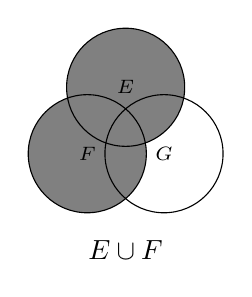
\begin{tikzpicture}[scale=0.75]
    \fill[fill=black!50] ( 90:.75) circle (1) (210:.75) circle (1);
    \foreach \a/\l in {90/E,210/F,330/G} {
        \path[draw] ++(\a:.75) circle (1) node {$\scriptstyle \l$};
    }
    \node at (0, -2) {$E \cup F$};
    \end{tikzpicture}
    \hspace{1em}
    \begin{tikzpicture}[scale=0.75]
    \fill[fill=black!50] (90:.75) circle (1);
    \scope[even odd rule]
        \clip ( 90:.75) circle (1) (330:.75) circle (1);
        \clip (210:.75) circle (1) (330:.75) circle (1);
        \fill[fill=black!50] (330:.75) circle (1);
    \endscope
    \foreach \a/\l in {90/E,210/F,330/G} {
        \path[draw] ++(\a:.75) circle (1) node {$\scriptstyle \l$};
    }
    \node at (0, -2) {$E \cup F^\complement $};
    \end{tikzpicture}
    \]
    su intersección
    \[
    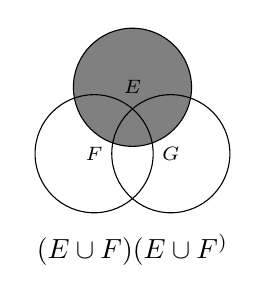
\begin{tikzpicture}[scale=0.75]
    \fill[fill=black!50] (90:.75) circle (1);
    \foreach \a/\l in {90/E,210/F,330/G} {
        \path[draw] ++(\a:.75) circle (1) node {$\scriptstyle \l$};
    }
    \node at (0, -2) {$(E \cup F) (E \cup F^\complement )$};
    \end{tikzpicture}
    \]
    \item to prove DeMorgan’s laws for events $E$ and $F$. (prove $(E \cup F)^\complement  = E^\complement F^\complement $, and $(EF)^\complement  = E^\complement  \cup F^\complement $)

    \begin{proof}[Demostración] $(E \cup F)^\complement  = E^\complement F^\complement $
        \[
        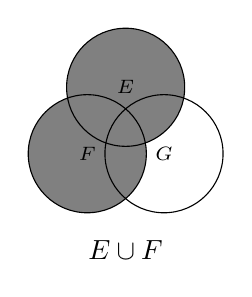
\begin{tikzpicture}[scale=0.75]
        \fill[fill=black!50] ( 90:.75) circle (1) (210:.75) circle (1);
        \foreach \a/\l in {90/E,210/F,330/G} {
            \path[draw] ++(\a:.75) circle (1) node {$\scriptstyle \l$};
        }
        \node at (0, -2) {$E \cup F$};
        \end{tikzpicture}
        \]
        su complemento
        \[
        \begin{tikzpicture}[scale=0.75]
        \scope[even odd rule]
            \clip ( 90:.75) circle (1) (330:.75) circle (1);
            \clip (210:.75) circle (1) (330:.75) circle (1);
            \fill[fill=black!50] (330:.75) circle (1);
        \endscope
        \foreach \a/\l in {90/E,210/F,330/G} {
            \path[draw] ++(\a:.75) circle (1) node {$\scriptstyle \l$};
        }
        \node at (0, -2) {$(E \cup F)^\complement $};
        \end{tikzpicture}
        \]
        \[
        \begin{tikzpicture}[scale=0.75]
        \scope[even odd rule]
            \clip (210:.75) circle (1) (330:.75) circle (1);
            \clip ( 90:.75) circle (1) (210:.75) circle (1);
            \fill[fill=black!50] (210:.75) circle (1);
        \endscope
        \scope[even odd rule]
            \clip ( 90:.75) circle (1) (330:.75) circle (1);
            \fill[fill=black!50] (330:.75) circle (1);
        \endscope
        \foreach \a/\l in {90/E,210/F,330/G} {
            \path[draw] ++(\a:.75) circle (1) node {$\scriptstyle \l$};
        }
        \node at (0, -2) {$E^\complement $};
        \end{tikzpicture}
        \hspace{1em}
        \begin{tikzpicture}[scale=0.75]
        \scope[even odd rule]
            \clip ( 90:.75) circle (1) (210:.75) circle (1);
            \clip (330:.75) circle (1) ( 90:.75) circle (1);
            \fill[fill=black!50] ( 90:.75) circle (1);
        \endscope
        \scope[even odd rule]
            \clip (210:.75) circle (1) (330:.75) circle (1);
            \fill[fill=black!50] (330:.75) circle (1);
        \endscope
        \foreach \a/\l in {90/E,210/F,330/G} {
            \path[draw] ++(\a:.75) circle (1) node {$\scriptstyle \l$};
        }
        \node at (0, -2) {$F^\complement $};
        \end{tikzpicture}
        \]
        su intersección
        \[
        \begin{tikzpicture}[scale=0.75]
        \scope[even odd rule]
            \clip ( 90:.75) circle (1) (330:.75) circle (1);
            \clip (210:.75) circle (1) (330:.75) circle (1);
            \fill[fill=black!50] (330:.75) circle (1);
        \endscope
        \foreach \a/\l in {90/E,210/F,330/G} {
            \path[draw] ++(\a:.75) circle (1) node {$\scriptstyle \l$};
        }
        \node at (0, -2) {$E^\complement  F^\complement $};
        \end{tikzpicture}
        \qedhere \]
    \end{proof}
    
    
    \begin{proof}[Demostración] $(EF)^\complement  = E^\complement  \cup F^\complement $
        \[
        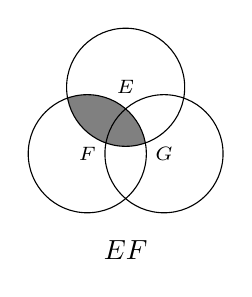
\begin{tikzpicture}[scale=0.75]
        \scope
            \clip (210:.75) circle (1);
            \fill[fill=black!50] ( 90:.75) circle (1);
        \endscope
        \foreach \a/\l in {90/E,210/F,330/G} {
            \path[draw] ++(\a:.75) circle (1) node {$\scriptstyle \l$};
        }
        \node at (0, -2) {$EF$};
        \end{tikzpicture}
        \]
        su complemento
        \[
        \begin{tikzpicture}[scale=0.75]
        \scope[even odd rule]
            \clip ( 90:.75) circle (1) (210:.75) circle (1);
            \fill[fill=black!50] (210:.75) circle (1);
        \endscope
        \scope[even odd rule]
            \clip ( 90:.75) circle (1) (210:.75) circle (1);
            \fill[fill=black!50] (90:.75) circle (1);
        \endscope
        \scope[even odd rule]
            \clip ( 90:.75) circle (1) (330:.75) circle (1);
            \clip (210:.75) circle (1) (330:.75) circle (1);
            \fill[fill=black!50] (330:.75) circle (1);
        \endscope
        \foreach \a/\l in {90/E,210/F,330/G} {
            \path[draw] ++(\a:.75) circle (1) node {$\scriptstyle \l$};
        }
        \node at (0, -2) {$(EF)^\complement $};
        \end{tikzpicture}
        \]
        \[
        \begin{tikzpicture}[scale=0.75]
        \scope[even odd rule]
            \clip (210:.75) circle (1) (330:.75) circle (1);
            \clip ( 90:.75) circle (1) (210:.75) circle (1);
            \fill[fill=black!50] (210:.75) circle (1);
        \endscope
        \scope[even odd rule]
            \clip ( 90:.75) circle (1) (330:.75) circle (1);
            \fill[fill=black!50] (330:.75) circle (1);
        \endscope
        \foreach \a/\l in {90/E,210/F,330/G} {
            \path[draw] ++(\a:.75) circle (1) node {$\scriptstyle \l$};
        }
        \node at (0, -2) {$E^\complement $};
        \end{tikzpicture}
        \hspace{1em}
        \begin{tikzpicture}[scale=0.75]
        \scope[even odd rule]
            \clip ( 90:.75) circle (1) (210:.75) circle (1);
            \clip (330:.75) circle (1) ( 90:.75) circle (1);
            \fill[fill=black!50] ( 90:.75) circle (1);
        \endscope
        \scope[even odd rule]
            \clip (210:.75) circle (1) (330:.75) circle (1);
            \fill[fill=black!50] (330:.75) circle (1);
        \endscope
        \foreach \a/\l in {90/E,210/F,330/G} {
            \path[draw] ++(\a:.75) circle (1) node {$\scriptstyle \l$};
        }
        \node at (0, -2) {$F^\complement $};
        \end{tikzpicture}
        \]
        su unión
        \[
        \begin{tikzpicture}[scale=0.75]
        \scope[even odd rule]
            \clip ( 90:.75) circle (1) (210:.75) circle (1);
            \fill[fill=black!50] (210:.75) circle (1);
        \endscope
        \scope[even odd rule]
            \clip ( 90:.75) circle (1) (210:.75) circle (1);
            \fill[fill=black!50] (90:.75) circle (1);
        \endscope
        \scope[even odd rule]
            \clip ( 90:.75) circle (1) (330:.75) circle (1);
            \clip (210:.75) circle (1) (330:.75) circle (1);
            \fill[fill=black!50] (330:.75) circle (1);
        \endscope
        \foreach \a/\l in {90/E,210/F,330/G} {
            \path[draw] ++(\a:.75) circle (1) node {$\scriptstyle \l$};
        }
        \node at (0, -2) {$E^\complement  \cup F^\complement $};
        \end{tikzpicture} \qedhere
        \]
    \end{proof}
    
    
\end{enumerate}
